\chapter{State of the art}
\label{chap:2_sota}

This chapter delivers a review of the state of the art, to provide a general panorama of the problems and methods that this work addresses.\\

As it was previously introduced, this work is performed to explore the synergies on robotics and deep-learning-based visual perception. In this section, the current approaches and tools will be described in order to outline a general panorama where this work may be framed.\\

The problem to be addressed is to \textit{get a robot with a camera to follow a person}. This problem can be split into several steps, where different approaches have been previously proposed. These steps will be covered in the following sections.
	
\section{Visual person detection}
\label{sec:2_detection}
One of the most common approaches is known as the \textit{Viola-Jones} detector \cite{violajones}. This algorithm relies on a \textit{rigid body model}, which fits a specific shape. On a grayscale image, this shape can be typically distinguished by means of the pixel intensity levels. Although this method was originally designed to detect faces, the rigid body model allows to generalize its usage for detecting different objects, such as persons. With this purpose, several spatial filters called \textit{Haar features} (\autoref{fig:2_haarfeats}) are introduced: these are used across the image looking for the intensity pattern of each template, which should resemble a part of the rigid body. Since this detector provides a weak decision by itself, several filters (previously chosen in a training process) are combined on a \textit{boosted cascade} (\autoref{fig:2_violajones_boost}). A person is detected if the weighted combination of several filters are triggered inside a certain area, which is decided to potentially contain a person \cite{diapos_cv_clasif}.

\begin{figure}[h]
	\centering
	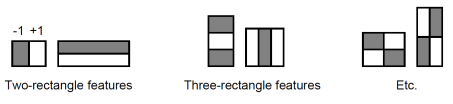
\includegraphics[width=0.7\linewidth]{haar_feats}
	\caption{Haar features: some examples \cite{diapos_cv_clasif}.}
	\label{fig:2_haarfeats}
\end{figure}

\begin{figure}[h]
	\centering
	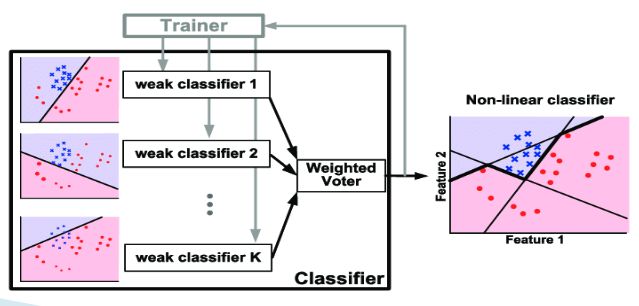
\includegraphics[width=0.7\linewidth]{boosted_cascade}
	\caption{Boosted weak classifiers \cite{diapos_cv_clasif}.}
	\label{fig:2_violajones_boost}
\end{figure}

The open-source standard image processing library, OpenCV, includes pre-trained models\footnote{\url{https://github.com/opencv/opencv/blob/master/data/haarcascades}}, which can be directly used with their Viola-Jones implementation. Scale invariance can be achieved evaluating the image at multiple scales on runtime.


Another common approach for person detection is based on HoG (\textit{Histograms of Gradients}) \cite{hog_detection}. This method computes local features by means of the intensity gradients across the image, and quantizes them according to their orientations (creating a histogram of oriented gradients for an image block), as it can be seen on \autoref{fig:2_hog}.\\



These gradients are collected in $64 \times 128$ windows, and treated as features. These features are evaluated by a linear SVM (\textit{Support Vector Machine}), which is trained to classify a window as \textit{person/non-person}. \autoref{fig:2_hog} shows the average gradient patch for a person (the direction of each gradient is not shown). A visual inspection immediately resembles the shape of a person standing up. Thus, this detector will yield the best performance when the person to be detected stands in that specific pose. This template allows as well to retain the gradients placed in the edges of the body (positive gradients), and discard those inside the body (negative gradients), weighting them according to their position inside the mentioned template.


\begin{figure}[h]
	\centering
	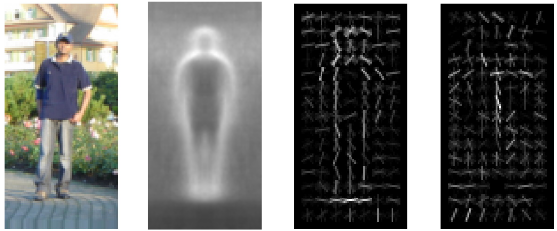
\includegraphics[width=0.7\linewidth]{hog}
	\caption{Example of the HoG computed for a person. From left to right: original image, average magnitude of the gradients on a person, directions weighted positive and negative gradients found in the input image. Image from \cite{hog_detection}.}
	\label{fig:2_hog}
\end{figure}




These methods, among several more, have been the state-of-the-art techniques: the cornerstone are the image gradients, which can be computed with a high efficiency, represented in a compact way by means of a histogram and provide decent performance. Their main drawback is the \textit{generalization} capability, as a successful detection is highly dependent on the person pose. However, in the latest advances, the detection techniques have moved towards the spreading paradigm: \textit{deep learning}, especially the most salient tools on image processing: CNNs (\textit{convolutional neural networks}).\\

CNNs are based on standard neural networks, which combine lots of neurons or \textit{perceptrons} organizing them into layers. These perceptrons (\autoref{fig:2_perceptron}) implement simple non-linear operations, that allow to extract (after a proper training process) abstract features, which gain in complexity when the number of internal layers increases. When a neural network is composed by many \textit{hidden} layers (in addition to the input/output ones), it is placed into the \textit{deep learning} paradigm (\autoref{fig:2_deep_learning}), as opposed to \textit{shallow learning}.

\begin{figure}[h]
	\centering
	\begin{subfigure}[t]{0.35\linewidth}
		\centering
		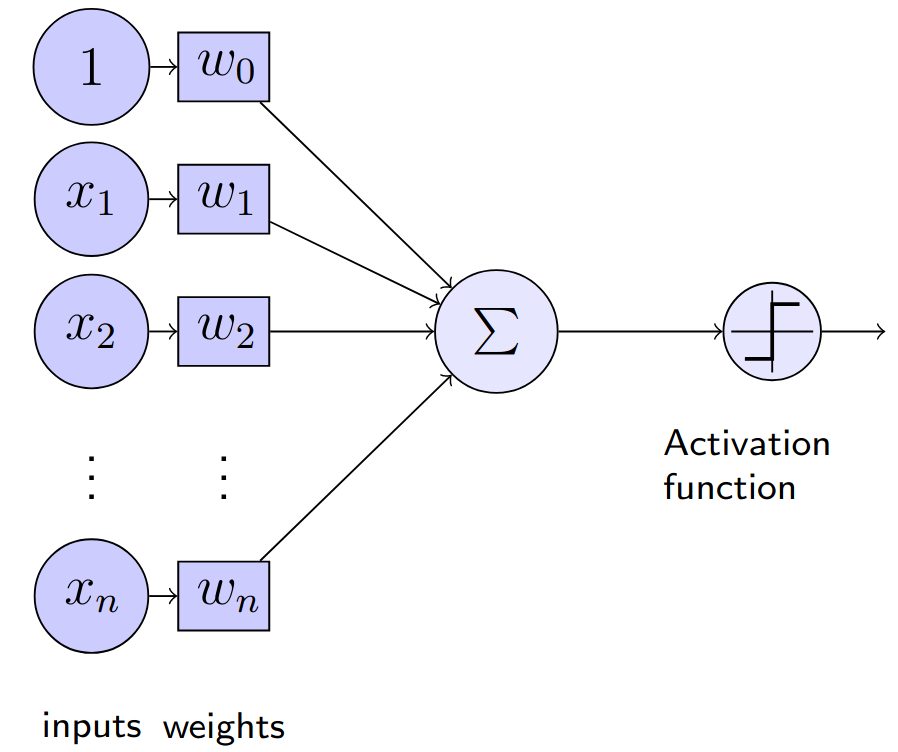
\includegraphics[width=0.95\linewidth]{perceptron}
		\caption{Basic unit of a neural network: the perceptron (source: \cite{tfg}).}
		\label{fig:2_perceptron}
	\end{subfigure}
	\begin{subfigure}[t]{0.5\linewidth}
		\centering
		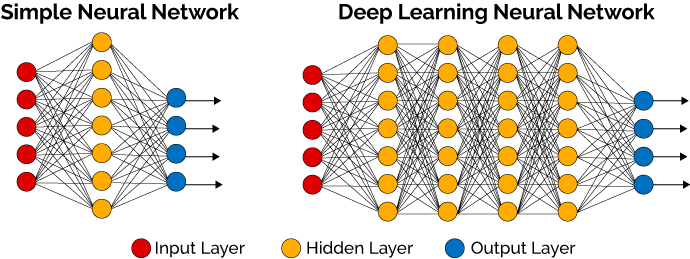
\includegraphics[width=0.99\linewidth]{deep_learning}
		\caption{Standard neural network vs. deep neural network (source: \cite{tfg}).}
		\label{fig:2_deep_learning}
	\end{subfigure}
	\caption{Basis of deep neural networks. (a), schematic of a perceptron. (b), increment on the number of hidden layers on deep learning approaches.}
	\label{fig:2_dnns}
\end{figure}


Based on this approach, and taking advantage of the \textit{spatial correlation} when the signal to process is an image, a neural network can be modified to implement a different operation on each perceptron: a \textit{convolution} (\autoref{fig:2_convolution}).

\begin{figure}[h]
	\centering
	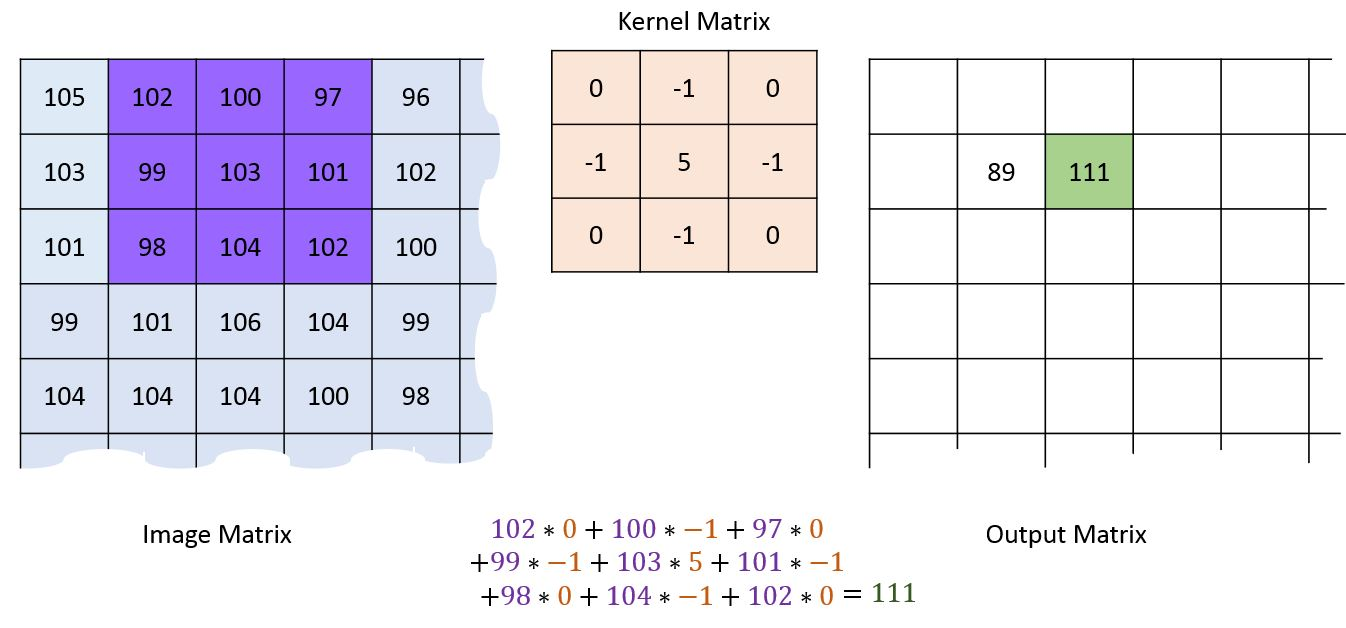
\includegraphics[width=0.7\linewidth]{convolution}
	\caption{Convolution applied to an image, applying the mask (red) on a region  (purple) of the input image, storing the result on the mapping of the central pixel of the region (green). The computation is the sum weighted by the mask values (bottom) (source: \cite{tfg}).}
	\label{fig:2_convolution}
\end{figure}

As it can be seen on \autoref{fig:2_cnn}, convolutional units may be arranged conforming a set of layers to build \textit{feature extraction} stages (shown in red in the figure). Several layers can be concatenated, gaining in depth and obtaining more complex feature maps. These layers are finally followed by a detection/classification ensemble of \textit{dense} layers (shown in blue in the figure): a set of layers with standard perceptrons fully-connected among them, yielding a final output, dependent on the classification structure of the network.

\begin{figure}[h]
	\centering
	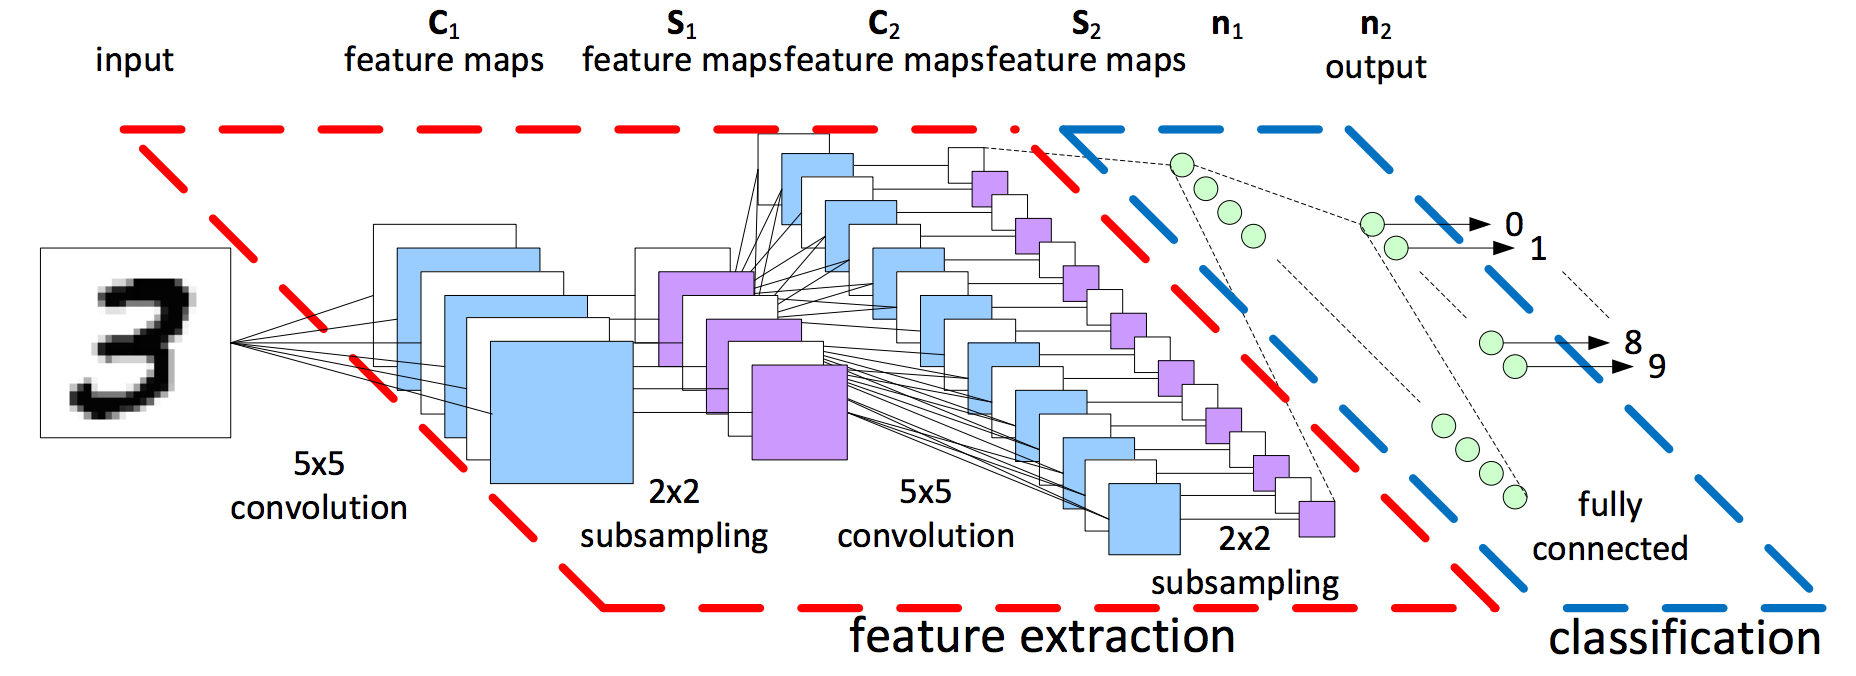
\includegraphics[width=0.9\linewidth]{cnn_architecture}
	\caption{Schematic of a digit classification CNN (source: \cite{tfg}).}
	\label{fig:2_cnn}
\end{figure}


In the case of object detection networks (the ones involved in this work), the output varies depending on the implementation, but it is generally composed of a set of \textit{(location, probability)} tuples, one for each class the network is capable of detecting. \autoref{fig:2_activation_maps} shows the activation maps of an object detection network, where the map presents higher values in the regions with high probability of containing the object of the class it is designed for. On a convolutional layer, each neuron computes several activation maps across the dimensions of the input data.

\begin{figure}[h]
	\centering
	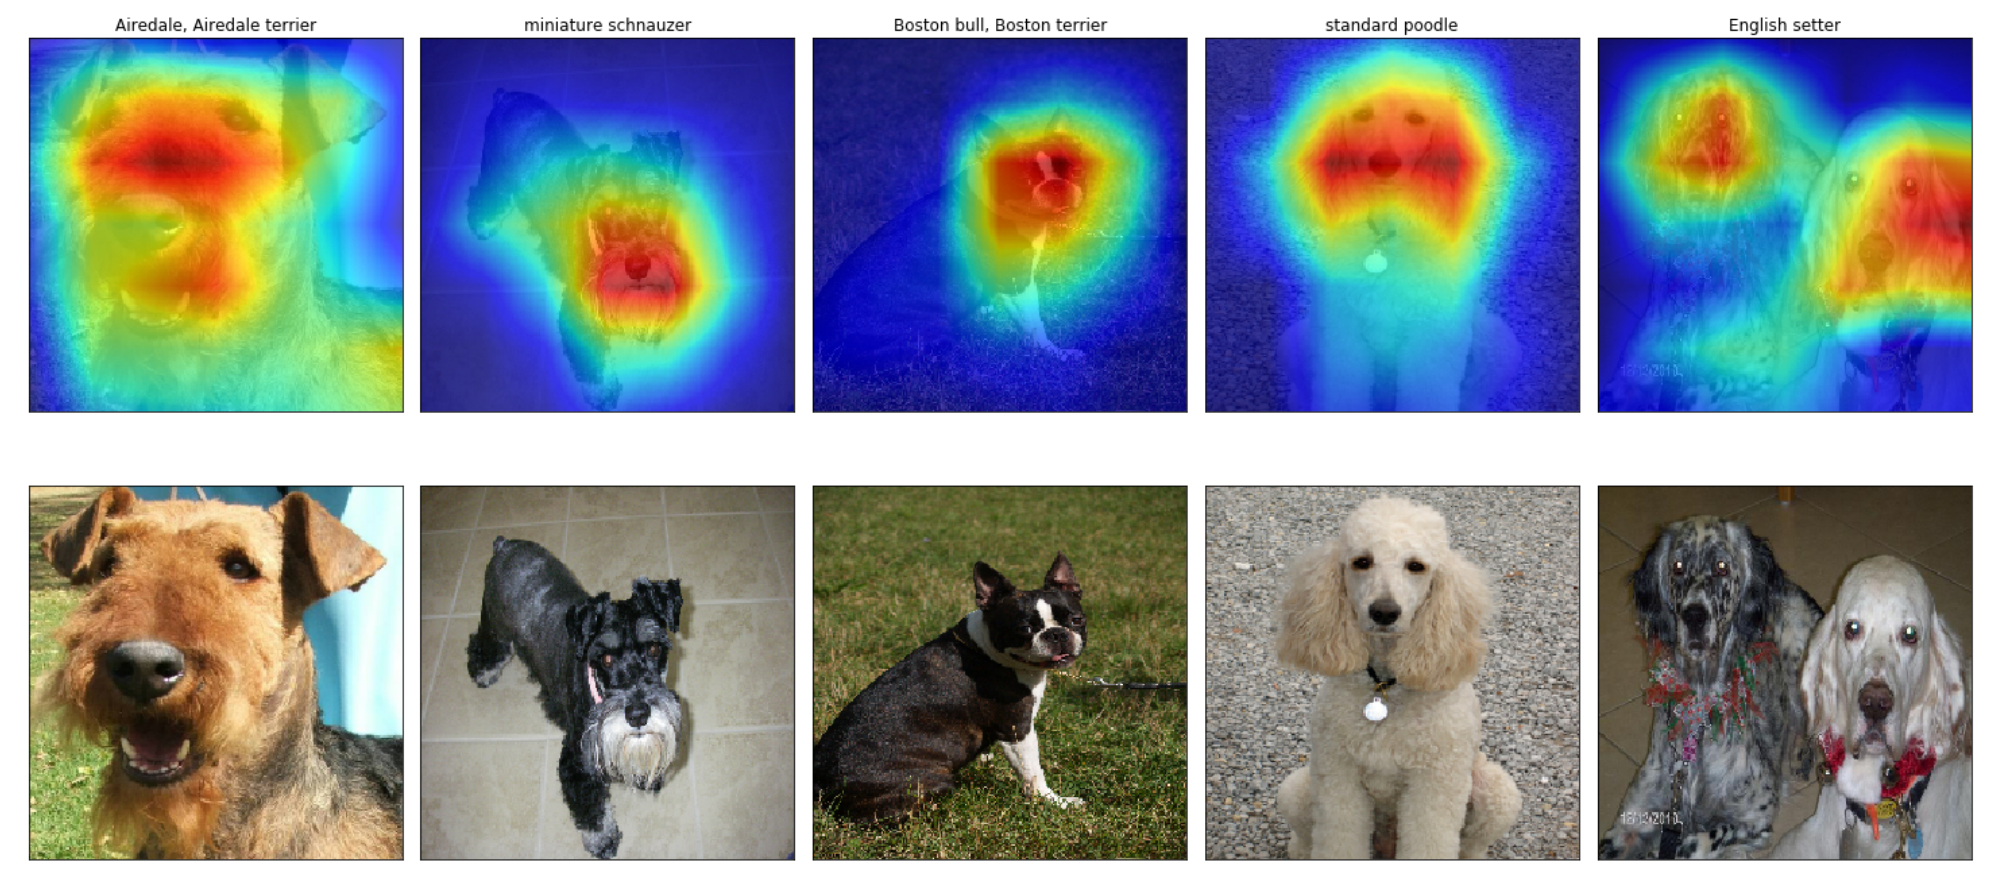
\includegraphics[width=0.9\linewidth]{activation_maps}
	\caption{Activation maps of a detection CNN searching for dogs on different images (source: \cite{tfg}).}
	\label{fig:2_activation_maps}
\end{figure}


One possible application of this concept is focused on what is called \textit{Region-based Convolutional Neural Networks} (R-CNNs) \cite{rcnn}, which require a previous step on the image called \textit{region proposal}. This step is devoted to find potential regions on the image to contain an object. This way, the challenge is to label these regions according to the objects contained inside, reducing the problem to a classification task. However, the process to find these regions and iterate over them makes the process too slow for real-time requirements, which are explicitly considered in our requirements. A notable effort has been made in later works \cite{fastrcnn} \cite{spp} to reduce this computation time.\\



\subsection{Single-Shot Multibox Detector (SSD)}
\label{sec:2_ssd}
Another outstanding object detection architecture is SSD (\textit{Single-Shot Multibox Detector}) \cite{ssd}. The main benefit from this architecture is the fact that it embeds all the required computations in a single neural network, reducing the complexity compared to other approaches requiring external region proposals, as it was explained above. This greatly reduces the computational time when the network has to process an image. The architecture can be seen at \autoref{fig:2_arch_ssd_yolo}, and can be split into several stages \cite{tfg}, namely:

\begin{description}
	
	\item[Reshape:] the first task to be addressed by the network is to reshape the input image(s) to a fixed size on which the rest of the layers work. In the case of an SSD detector, this shape is $n \times 300 \times 300 \times 3$ (being $n$ the size of the input batch, as $n$ images can be evaluated simultaneously on the neural network). Other image sizes might be used, however this one offers a good trade-off between performance and computational load.
	
	\item [Base network:] this first group of layers are reused from a typical image classification model, such as VGG-16 \cite{vgg16}. The first layers of this architecture are utilized in this design, truncated before the first classification layer. This way, the network can leverage the \textit{feature maps} from the classification network, in order to find objects inside the input image. Following the first part of the network, several convolutional layers are appended, decreasing in size. This has the objective of predict detections at multiple scales. One thing to mention at this point is that the base network can be a different one rather than VGG-16, such as a MobileNet \cite{mobilenet}, which is highly optimized for running on low-end devices. This is interesting as our embedded system will be limited in computing power. It will be revisited in future sections.
	
	\item[Box predictors:] for each layer in the base network, an image  convolution is performed, generating a small set (typically 3 or 4) of fixed-size \textit{anchors}, with varying aspect ratios for each cell on a grid over the activation map (\autoref{fig:2_ssd_generated_boxes}). As these maps have different sizes, the system is able to detect  objects in different scales. The anchors are then convolved with small filters (one per depth channel), which output confidence scores for each known class, and offsets for the generated bounding box. These scores are passed through a \textit{softmax} operation, that compresses them into a probability vector. Thus, for each detected object (on that scale), the network computes the score on every class and its estimated position inside the feature map (hence, in the image as well).
	
	\item [Postprocessor:] as several detections might be triggered in the same area for different classes and scales, a \textit{Non-Maximum-Supression} \cite{nms} operation is performed at the output of the network to retain the best boxes, under a combined criteria of detection score and IoU score (\textit{Intersection over Union}), which measures the overlapping quality between two bounding boxes, as it can be seen in \autoref{fig:2_iou}.
\end{description}


\begin{figure}[h]
	\centering
	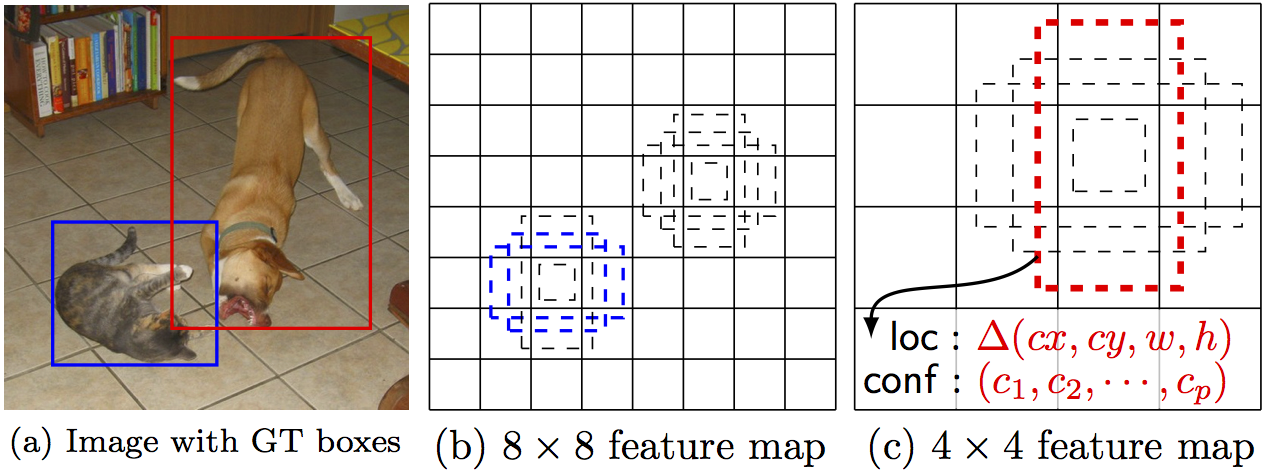
\includegraphics[width=0.7\linewidth]{ssd_generated_boxes}
	\caption{A set of boxes are generated centered on each point of every feature map \cite{ssd}.}
	\label{fig:2_ssd_generated_boxes}
\end{figure}

\begin{figure}[h]
	\centering
	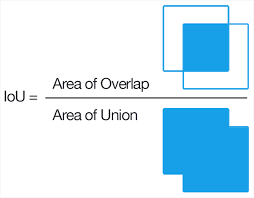
\includegraphics[width=0.4\linewidth]{iou}
	\caption{Graphical representation of the IoU score between two bounding boxes.}
	\label{fig:2_iou}
\end{figure}

\subsection{YOLO (You Only Look Once)}
\label{sec:2_yolo}
Another interesting approach is the YOLO (\textit{You Only Look Once}) system \cite{yolov1}. Its main advantage is its inference speed, due to the fact that it performs a single analysis on the entire image, dividing it into a grid of cells. Each cell predicts up to 5 boxes, containing an \textit{objectness score} (the predicted IoU of the proposal with an object, regardless its class), the coordinates of the bounding box, and a probability for the object belonging to each class. This design run faster than other methods \cite{yolov1}, however it presents a poor performance when detecting small objects.\\

This design was revisited in YOLO9000 \cite{yolov2}, introducing several improvements such as batch normalization at the input of the convolutional layers, or the concept of \textit{anchor boxes}: the box proposals follow a fixed set of aspect ratios, chosen previously using clustering on a training set. As it can be seen on \autoref{fig:2_yolov2_anchor_clustering}, limiting the proposal shapes to 5 fixed sizes improves the performance while maintaining a high IoU metric. A visual inspection shows that the selected anchors seem like a reasonable shape for the majority of the objects the network aims to detect. Additionally, the number of deep layers was increased from 26 layers to 30, and a semantic modeling is performed on the labels across different datasets, allowing the network to be trained in different datasets under a common semantic structure called \textit{WordTree} (\autoref{fig:2_yolov2_wordtree}).

\begin{figure}[h]
	\centering
	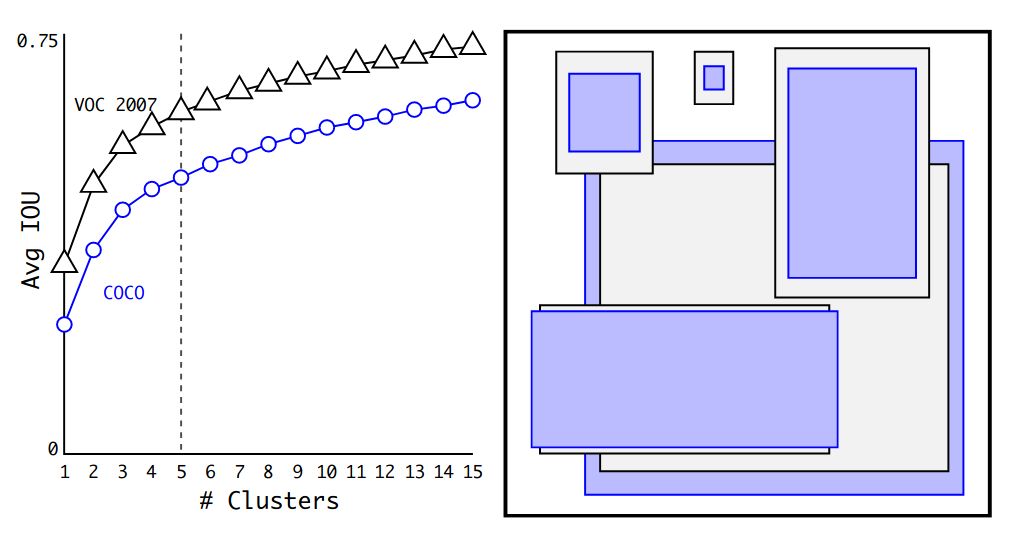
\includegraphics[width=0.6\linewidth]{yolov2_anchor_clustering}
	\caption{Result of the anchor k-means clustering on VOC and COCO for YOLO9000. Using $k=5$ anchor sizes on the right yields a good tradeoff between simplicity and improvement on the obtained IoU with respect to using $k-1$ clusters (source: \cite{yolov2}).}
	\label{fig:2_yolov2_anchor_clustering}
\end{figure}
%\vspace{20cm}


\begin{figure}[h]
	\centering
	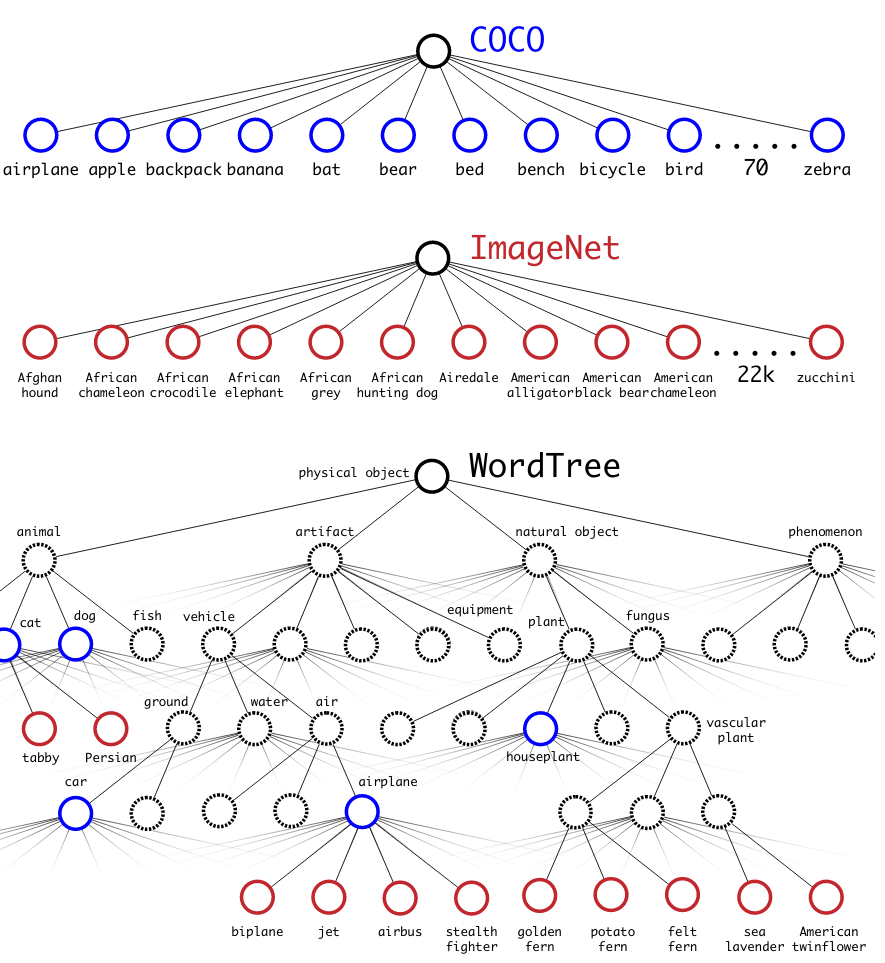
\includegraphics[width=0.6\linewidth]{yolov2_wordtree}
	\caption{Comparison between simple labeling structures (top) and a WordTree semantic grouping under categories (bottom). This allows to follow a dataset-agnostic training process as the labels can be combined using WordTree. Image from \cite{yolov2}.}
	\label{fig:2_yolov2_wordtree}
\end{figure}




The latest improvement of YOLO, YOLOv3 \cite{yolov3}, relies on residual networks \cite{resnets}, which tackle the problem of \textit{vanishing gradients} when the networks become deeper. The stacking of several layers results on gradients diminishing its value up to a point the arithmetical precision of the machine is not able to handle. The gradients are canceled, hindering the training process, as the first layers parameters take a substantially higher time to converge. The residual networks added in this revision of the design add shortcut connections across the layers, focusing the backpropagation gradients on the differences between the input and the output of the layer. As this reference states \cite{yolov3}, the combination of these residual layers and convolutional ones allows to train much deeper architectures (53 convolutional layers), capable of yielding a higher generalization. As in the SSD detectors, the YOLO architecture performs multi-scale detections, using 3 scales for splitting the feature maps into cell grids. A similar k-means clustering than in \autoref{fig:2_yolov2_anchor_clustering} is performed on the COCO dataset, selecting 9 anchor sizes instead of 5, and grouping them in 3 scales. Now, on each of the cells, 9 anchor bounding boxes are fit (3 anchor shapes $\times$ 3 scales). This aims to improve the poor performance of the previous version when dealing with small objects, as well as to produce better generalization: in the R-CNN \cite{rcnn} and the SSD \cite{ssd} the anchor shapes are hand-picked. These changes, with a tuning on the error function, conform the YOLOv3 improvements over the previous versions.\\

\vspace{5cm}

For each \textit{(anchor, cell, scale)} combination, YOLOv3 predicts:

\begin{itemize}
	\item The coordinates of the object within the anchor. Details can be visualized on \autoref{fig:2_yolo_output}.
	
	\item \textit{objectness} score, which is computed by means of a logistic regression in order to maximizing the probability of overlap with a ground truth bounding box with respect to that of any other prior anchor.
	
	\item 80 scores, as the original implementation is trained in the COCO dataset, which contains 80 classes. These classes might be overlapping (e.g. ``woman'' and ``person''). Thus, these scores are computed by independent logistic classifiers and are not passed through a \textit{softmax} operation.
\end{itemize}


\begin{figure}[h]
	\centering
	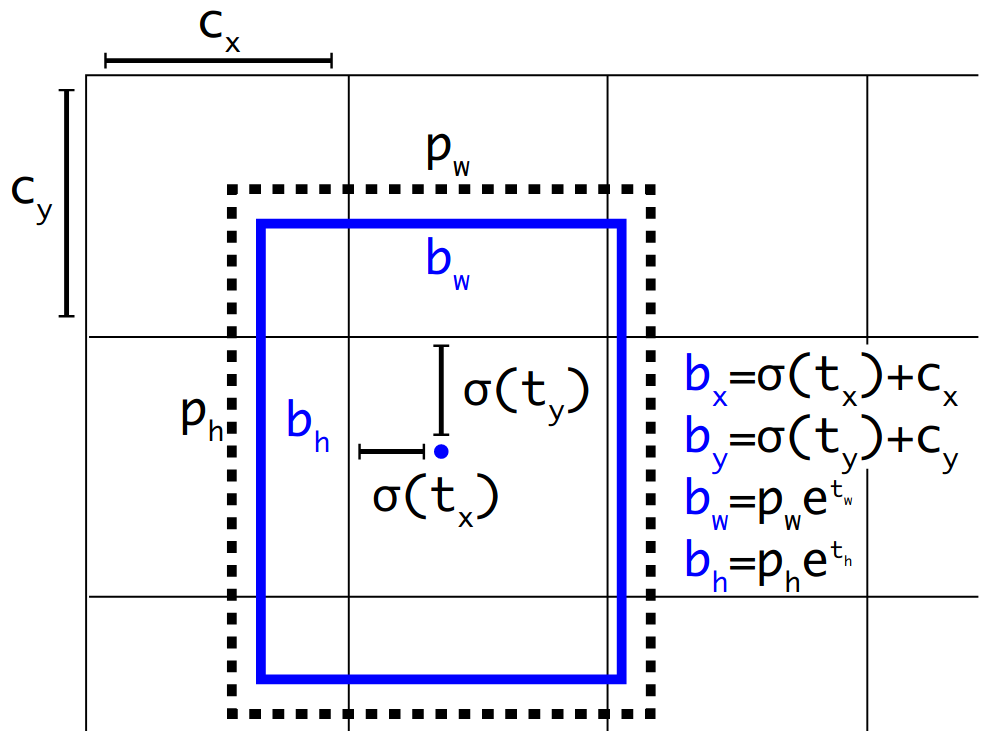
\includegraphics[width=0.5\linewidth]{yolo_outputs}
	\caption{Output on YOLO for each anchor and cell. The dashed line represents the prior anchor, while the blue line represents the detection which corrects that anchor.}
	\label{fig:2_yolo_output}
\end{figure}


The architecture of a YOLO-based detection network can be compared to that of a SSD-based one in \autoref{fig:2_arch_ssd_yolo}. This allows to see the fundamental difference in the feature extraction stage of each approach.

\begin{figure}[h]
	\centering
	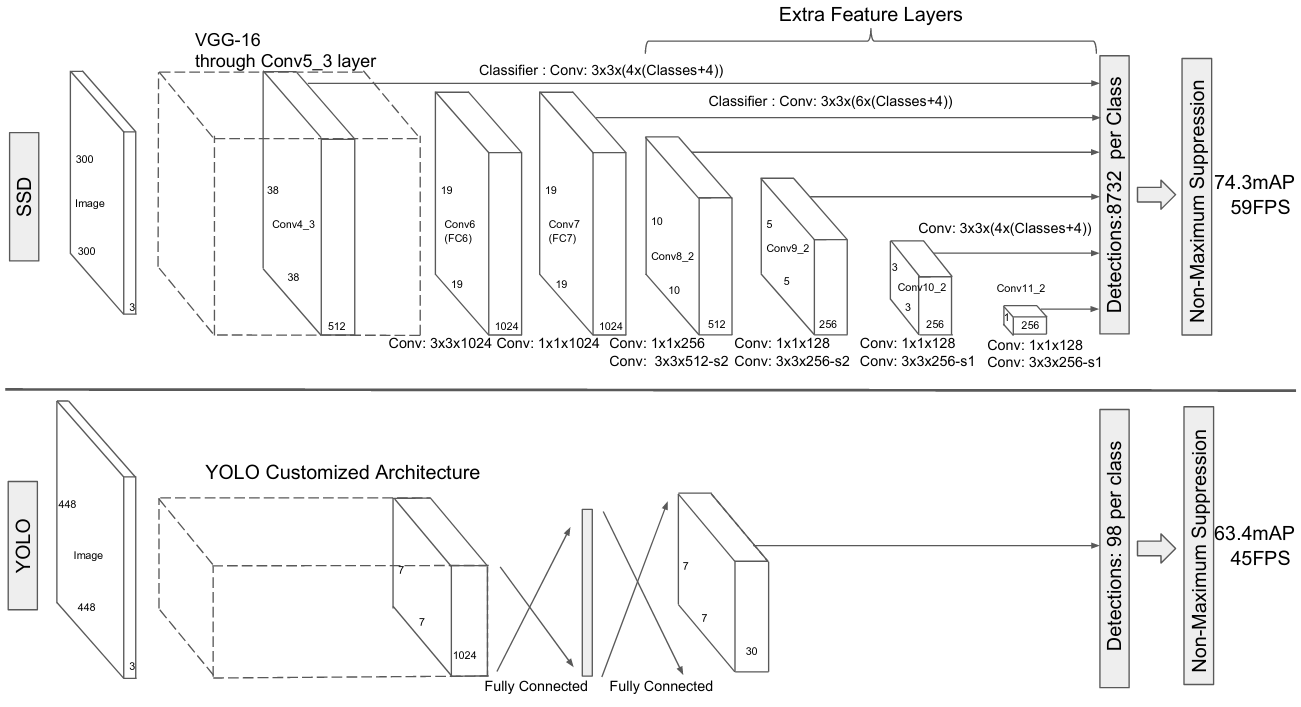
\includegraphics[width=0.8\linewidth]{arch_ssd_yolo}
	\caption{General architecture of a SSD network (top) and a YOLO one (bottom). Image from \cite{ssd}.}
	\label{fig:2_arch_ssd_yolo}
\end{figure}

\newpage
\section{Person identification}
\label{sec:2_ident}
On a controlled environment, where the only present person is the one to be followed, a person detection system could be enough for following purposes. However, in a real scenario, there might be several people inside the field of vision of the robot. This problem can be approached by means of a distinguishing feature of the person of interest, provided beforehand. One example is \cite{color_id}, which computes the color distribution of the person of interest, and later compares this distribution with the ones belonging to the different persons using the Bhattacharyya coefficient \cite{bhattacharyya} (a measurement of similarity between two probability distributions). This metric can be applied for computing the similarity between the color histograms of the reference person and the detected one. However, this system can be deceived replicating the color distribution of the person of interest: wearing similar clothes helps to reduce the distance between the histogram, leaving a chance to confound another person with the one to follow.\\

A more robust approach is to use the \textit{face} of the person as the discriminant feature, as its uniqueness makes it a good reference to identify the detected person. As it is summarized in \cite{dlib_review}, several applications extract facial \textit{landmarks} from the morphology of a given face (\autoref{fig:2_dlib_landmarks}), and use them to recognize the face, comparing it with a set of known faces and estimating the identity based on the distance to each known face. Some open-source libraries such as \texttt{dlib} and \texttt{OpenCV} provide algorithms to perform these processes.\\

\begin{figure}[h]
	\centering
	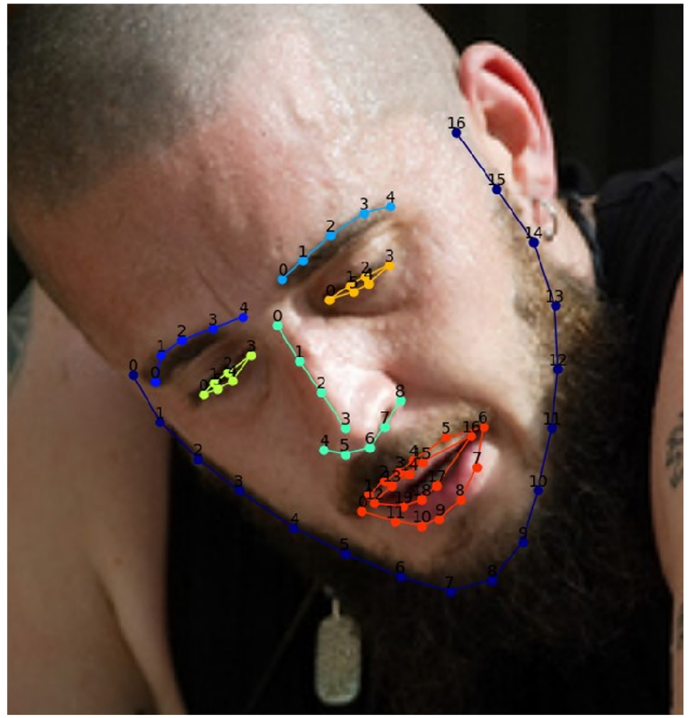
\includegraphics[width=0.6\linewidth]{dlib_landmarks}
	\caption{Facial landmarks are dependent of the face shape and morphology (image from \cite{dlib_review}).}
	\label{fig:2_dlib_landmarks}
\end{figure}


The intuition behind these methods are to \textit{project} the image of the face into a lower-dimensional space, which allows to extract significant features from each face. These features have to be consistent for the same face across different pose and lighting conditions (\autoref{fig:2_faces_poses}). An useful transformation when a dimensionality reduction is pursued is PCA (\textit{Principal Component Analysis}), a linear transformation that can be implemented to deal with the face recognition problem \cite{face_pca}.

\begin{figure}[h]
	\centering
	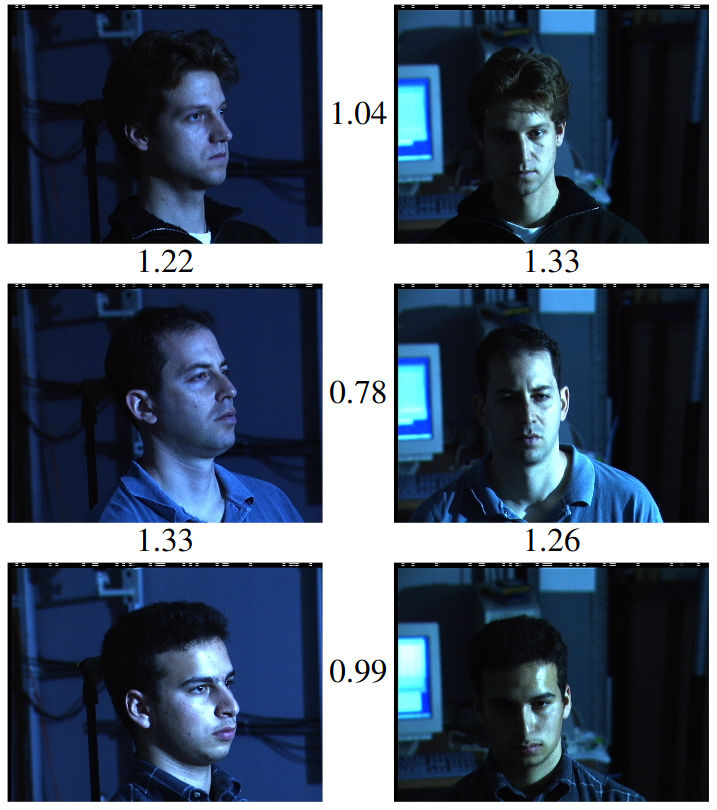
\includegraphics[width=0.40\linewidth]{face_poses}
	\caption{Examples of poses and light conditions across which the face projections are desired to be consistent for the same person (image from \cite{facenet}).}
	\label{fig:2_faces_poses}
\end{figure}
\vspace{4cm}
\subsection{Deep learning face identification: FaceNet}
\label{sec:2_facenet}
However, once again neural networks can be leveraged in order to achieve better performance: as the PCA is a linear operation, it could be learned by a single layer neural network. Thus, the introduction of deep networks can yield interesting results. The most relevant approach so far uses deep convolutional networks for performing this process \cite{facenet}, implementing an architecture called \textit{FaceNet}, which is partially based on the Inception \cite{inception} module, designed by Google researchers in order to greatly reduce the number of parameters in a neural network. What this network computes is called an \textit{embedding}, a projection of the input face image into a point in a 128-dimensional hyper-sphere. This allows to translate the identification into linear algebra terms, such as \textit{distance} between two faces, as well as clustering and applying unsupervised algorithms. The architecture can be visualized in \autoref{fig:2_facenet_architecture}. These networks can be trained using a loss function called \textit{triplet loss}, inspired by the work in \cite{lmnn_loss}. Given a training sample (\textit{anchor}), a \textit{positive} example (same class than the anchor) and a \textit{negative} example (different class than the anchor) are chosen, and the network is tuned to maximize the \textit{anchor-negative} embeddings distance, and minimize at the same time the \textit{anchor-positive} one (\autoref{fig:2_facenet_triplet_loss}).


\begin{figure}[h]
	\centering
	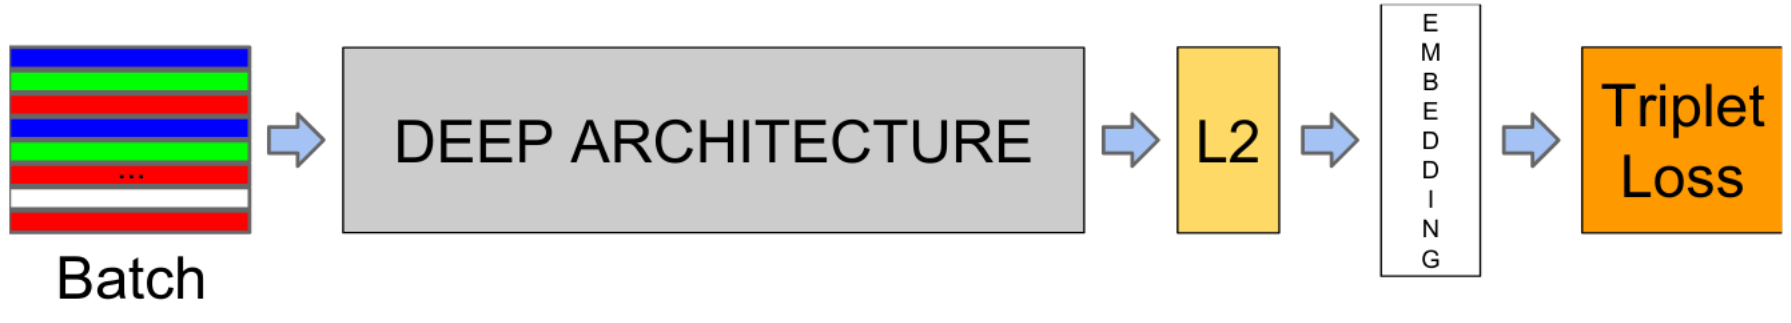
\includegraphics[width=0.7\linewidth]{facenet_architecture}
	\caption{Architecture of the FaceNet system (from \cite{facenet}).}
	\label{fig:2_facenet_architecture}
\end{figure}



\begin{figure}[h]
	\centering
	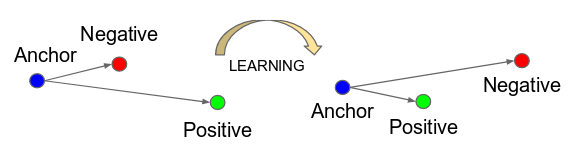
\includegraphics[width=0.7\linewidth]{facenet_triplet_loss}
	\caption{Triplet loss training. It minimizes the distance between an \emph{anchor} (current example) and a \emph{positive}, both of which have the same identity, and maximizes the distance between the \emph{anchor} and a \emph{negative} of a different identity (from \cite{facenet}).}
	\label{fig:2_facenet_triplet_loss}
\end{figure}


One thing to mention about the algorithms described above is that they perform the operations on the face image. Thus, a face detection is required for previously cropping the face of the person to be identified. One interesting approach using this technique is \textit{faced} \cite{faced}. This is a custom small ensemble of two neural networks, responsible to detect faces and correct the bounding boxes found. The main objective of the system is \textit{speed}, so the main detector architecture is based in YOLO \cite{yolov1}, and the second correction stage raises the precision achieved by the detector, achieving better results than a classical Haar approach, as illustrated on \autoref{fig:2_faced_vs_haar}. Further comparisons are performed on Chapter \ref{chap:4_results} between these two detection methods.

\begin{figure}[h]
	\centering
	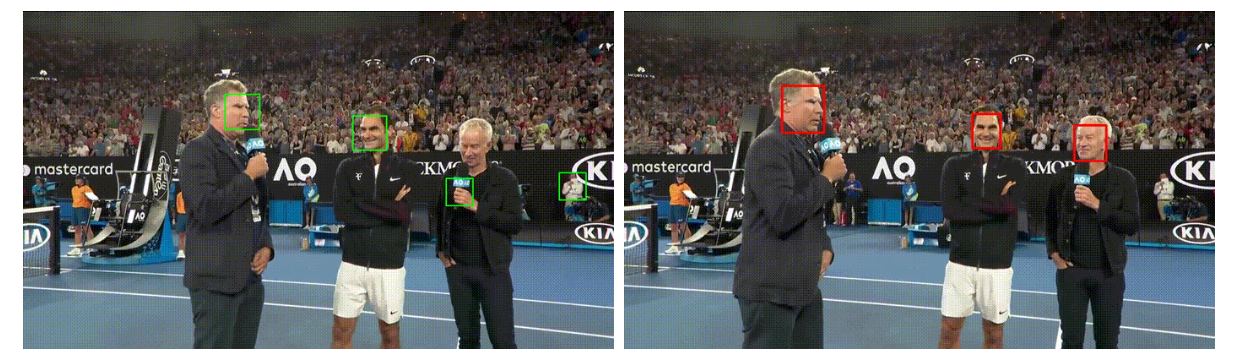
\includegraphics[width=0.8\linewidth]{faced_vs_haar}
	\caption{Classical Haar based face detector \cite{violajones} (left) vs. \textit{faced} (right). Image from \cite{faced}.}
	\label{fig:2_faced_vs_haar}
\end{figure}


\section{Embedded deployment}
\label{sec:2_embedded}
One of the requirements of this work is to be integrated in an autonomous robot. This imposes a power limitation on the algorithms to be deployed. Generally, the robotic systems are deployed using laptops connected to robots, as it was done in \cite{tfg} (\autoref{fig:2_real_tfg}).

\begin{figure}[h]
	\centering
	\begin{subfigure}[h]{0.4\linewidth}
		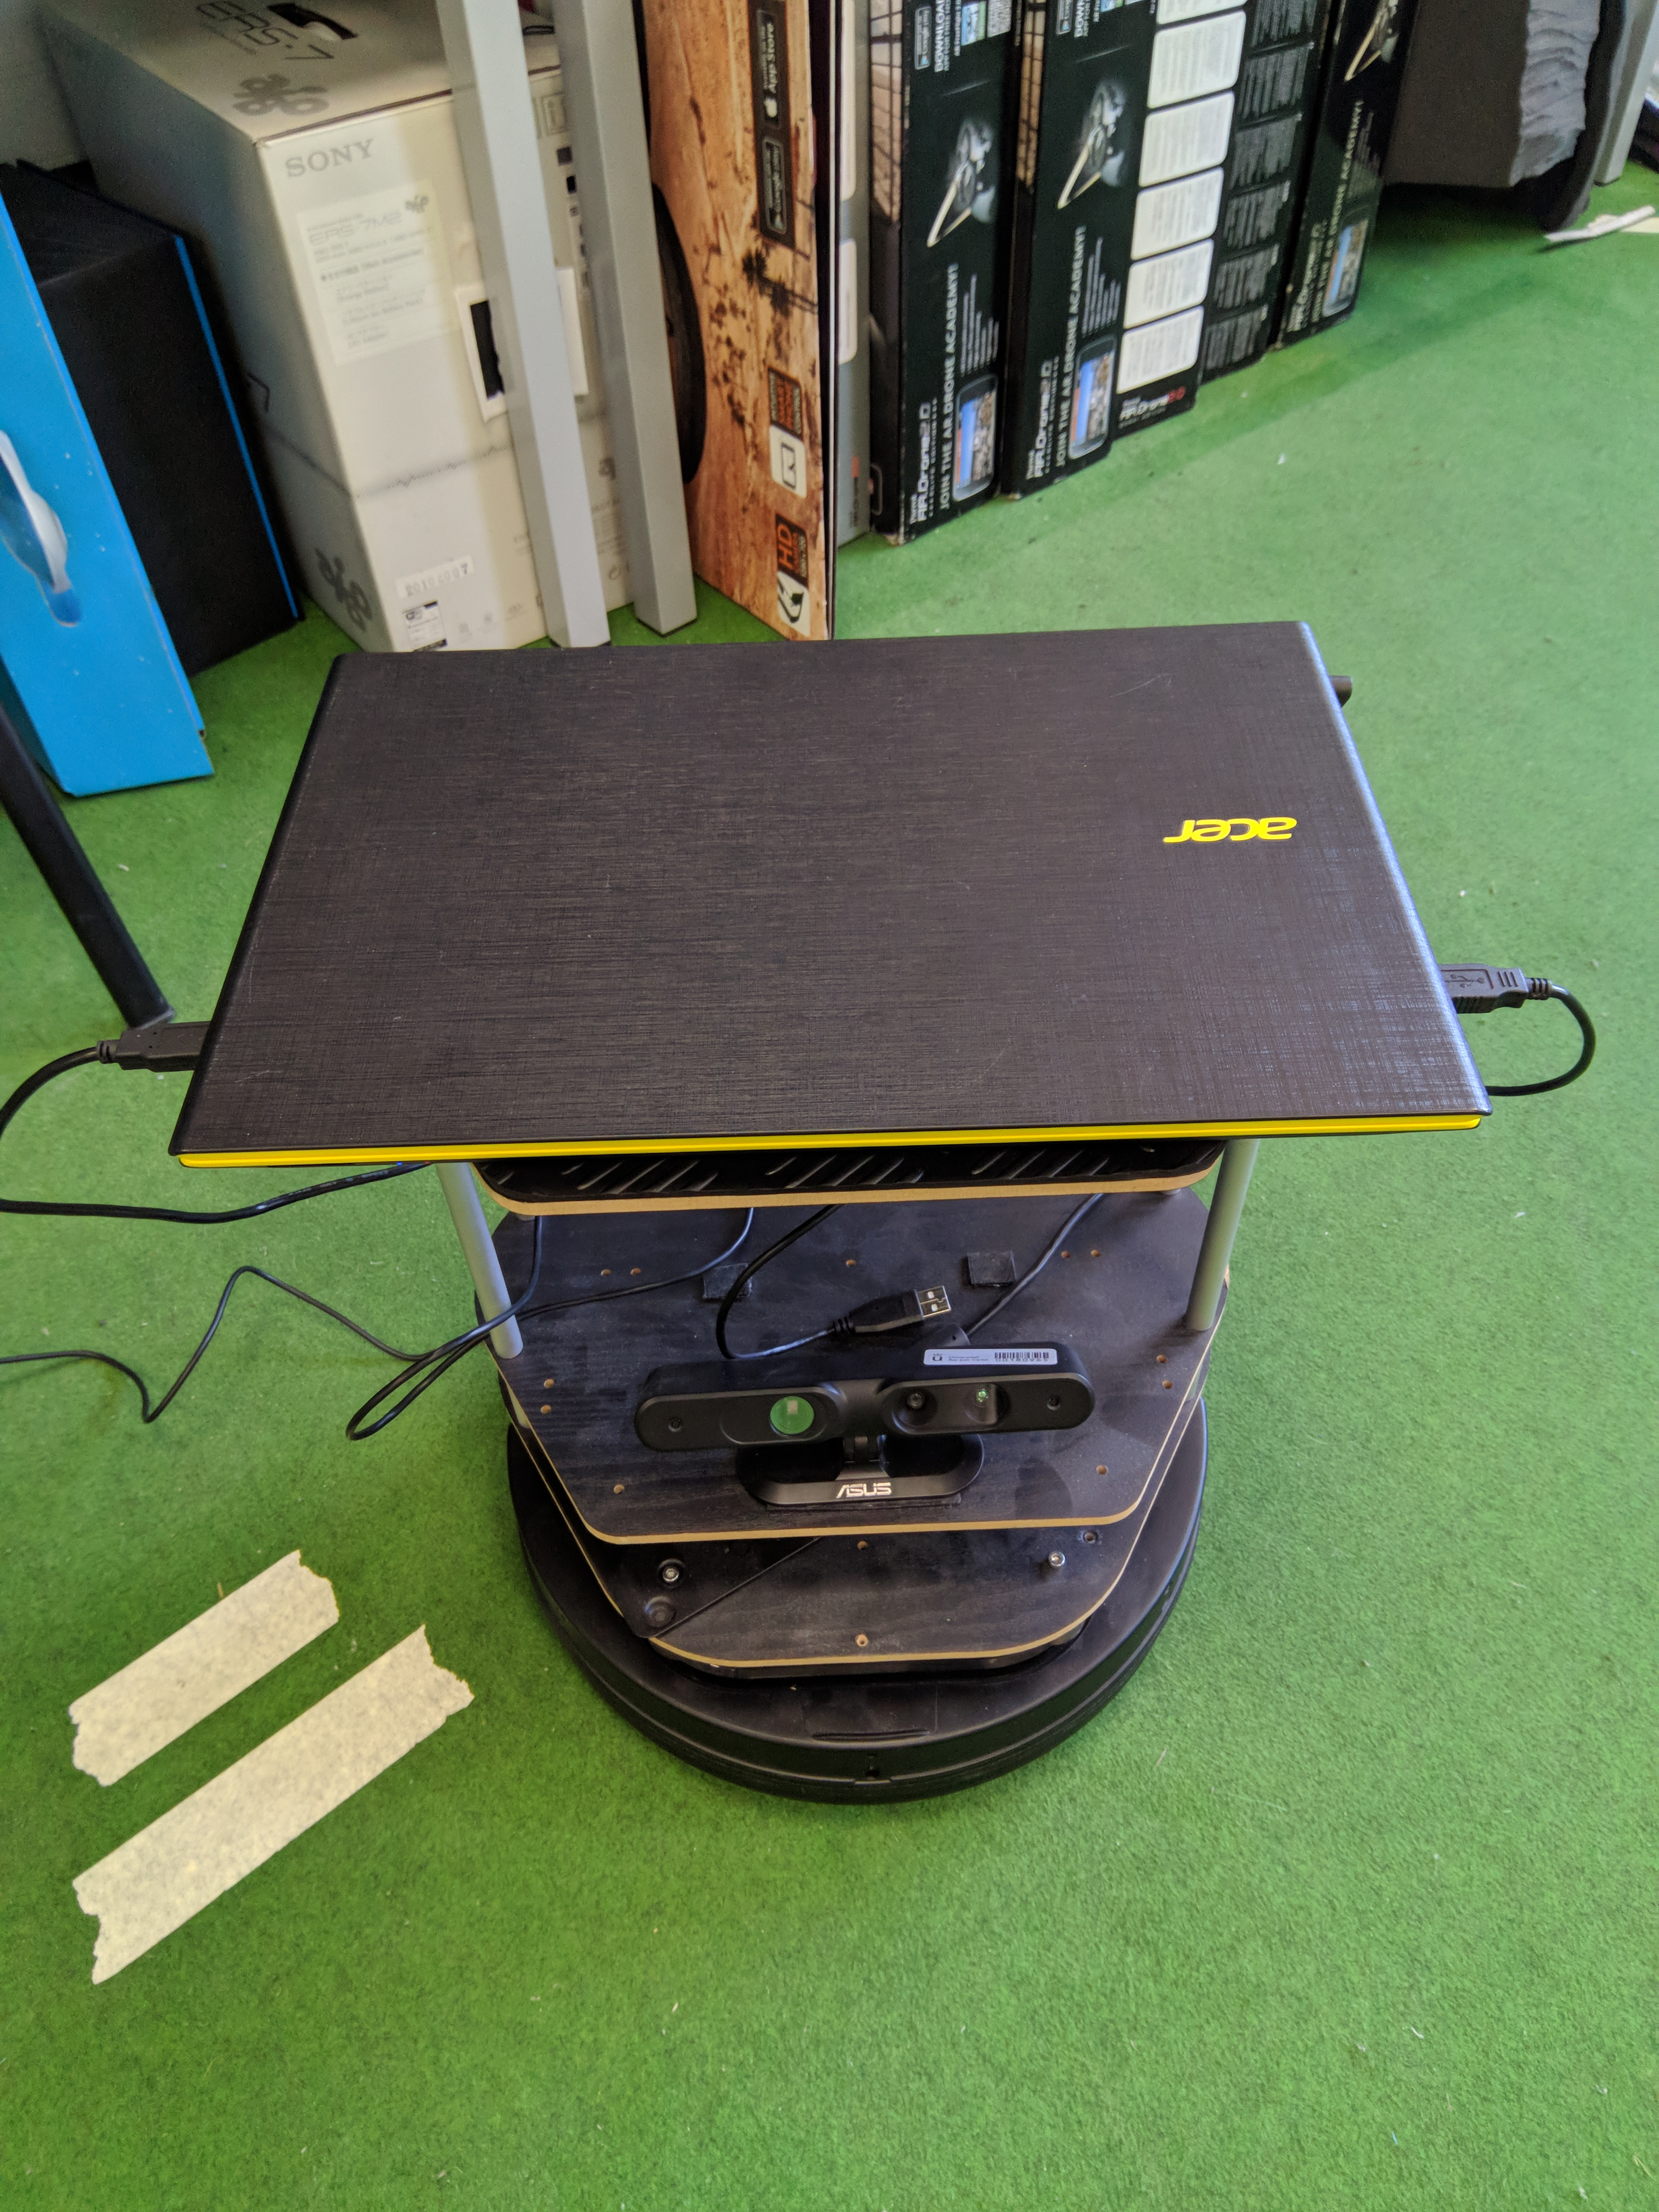
\includegraphics[width=1.9in]{tfg1}
		\caption{Frontal view.}
		\label{fig:2_turtlebot_front}
	\end{subfigure}
	\begin{subfigure}[h]{0.4\linewidth}
		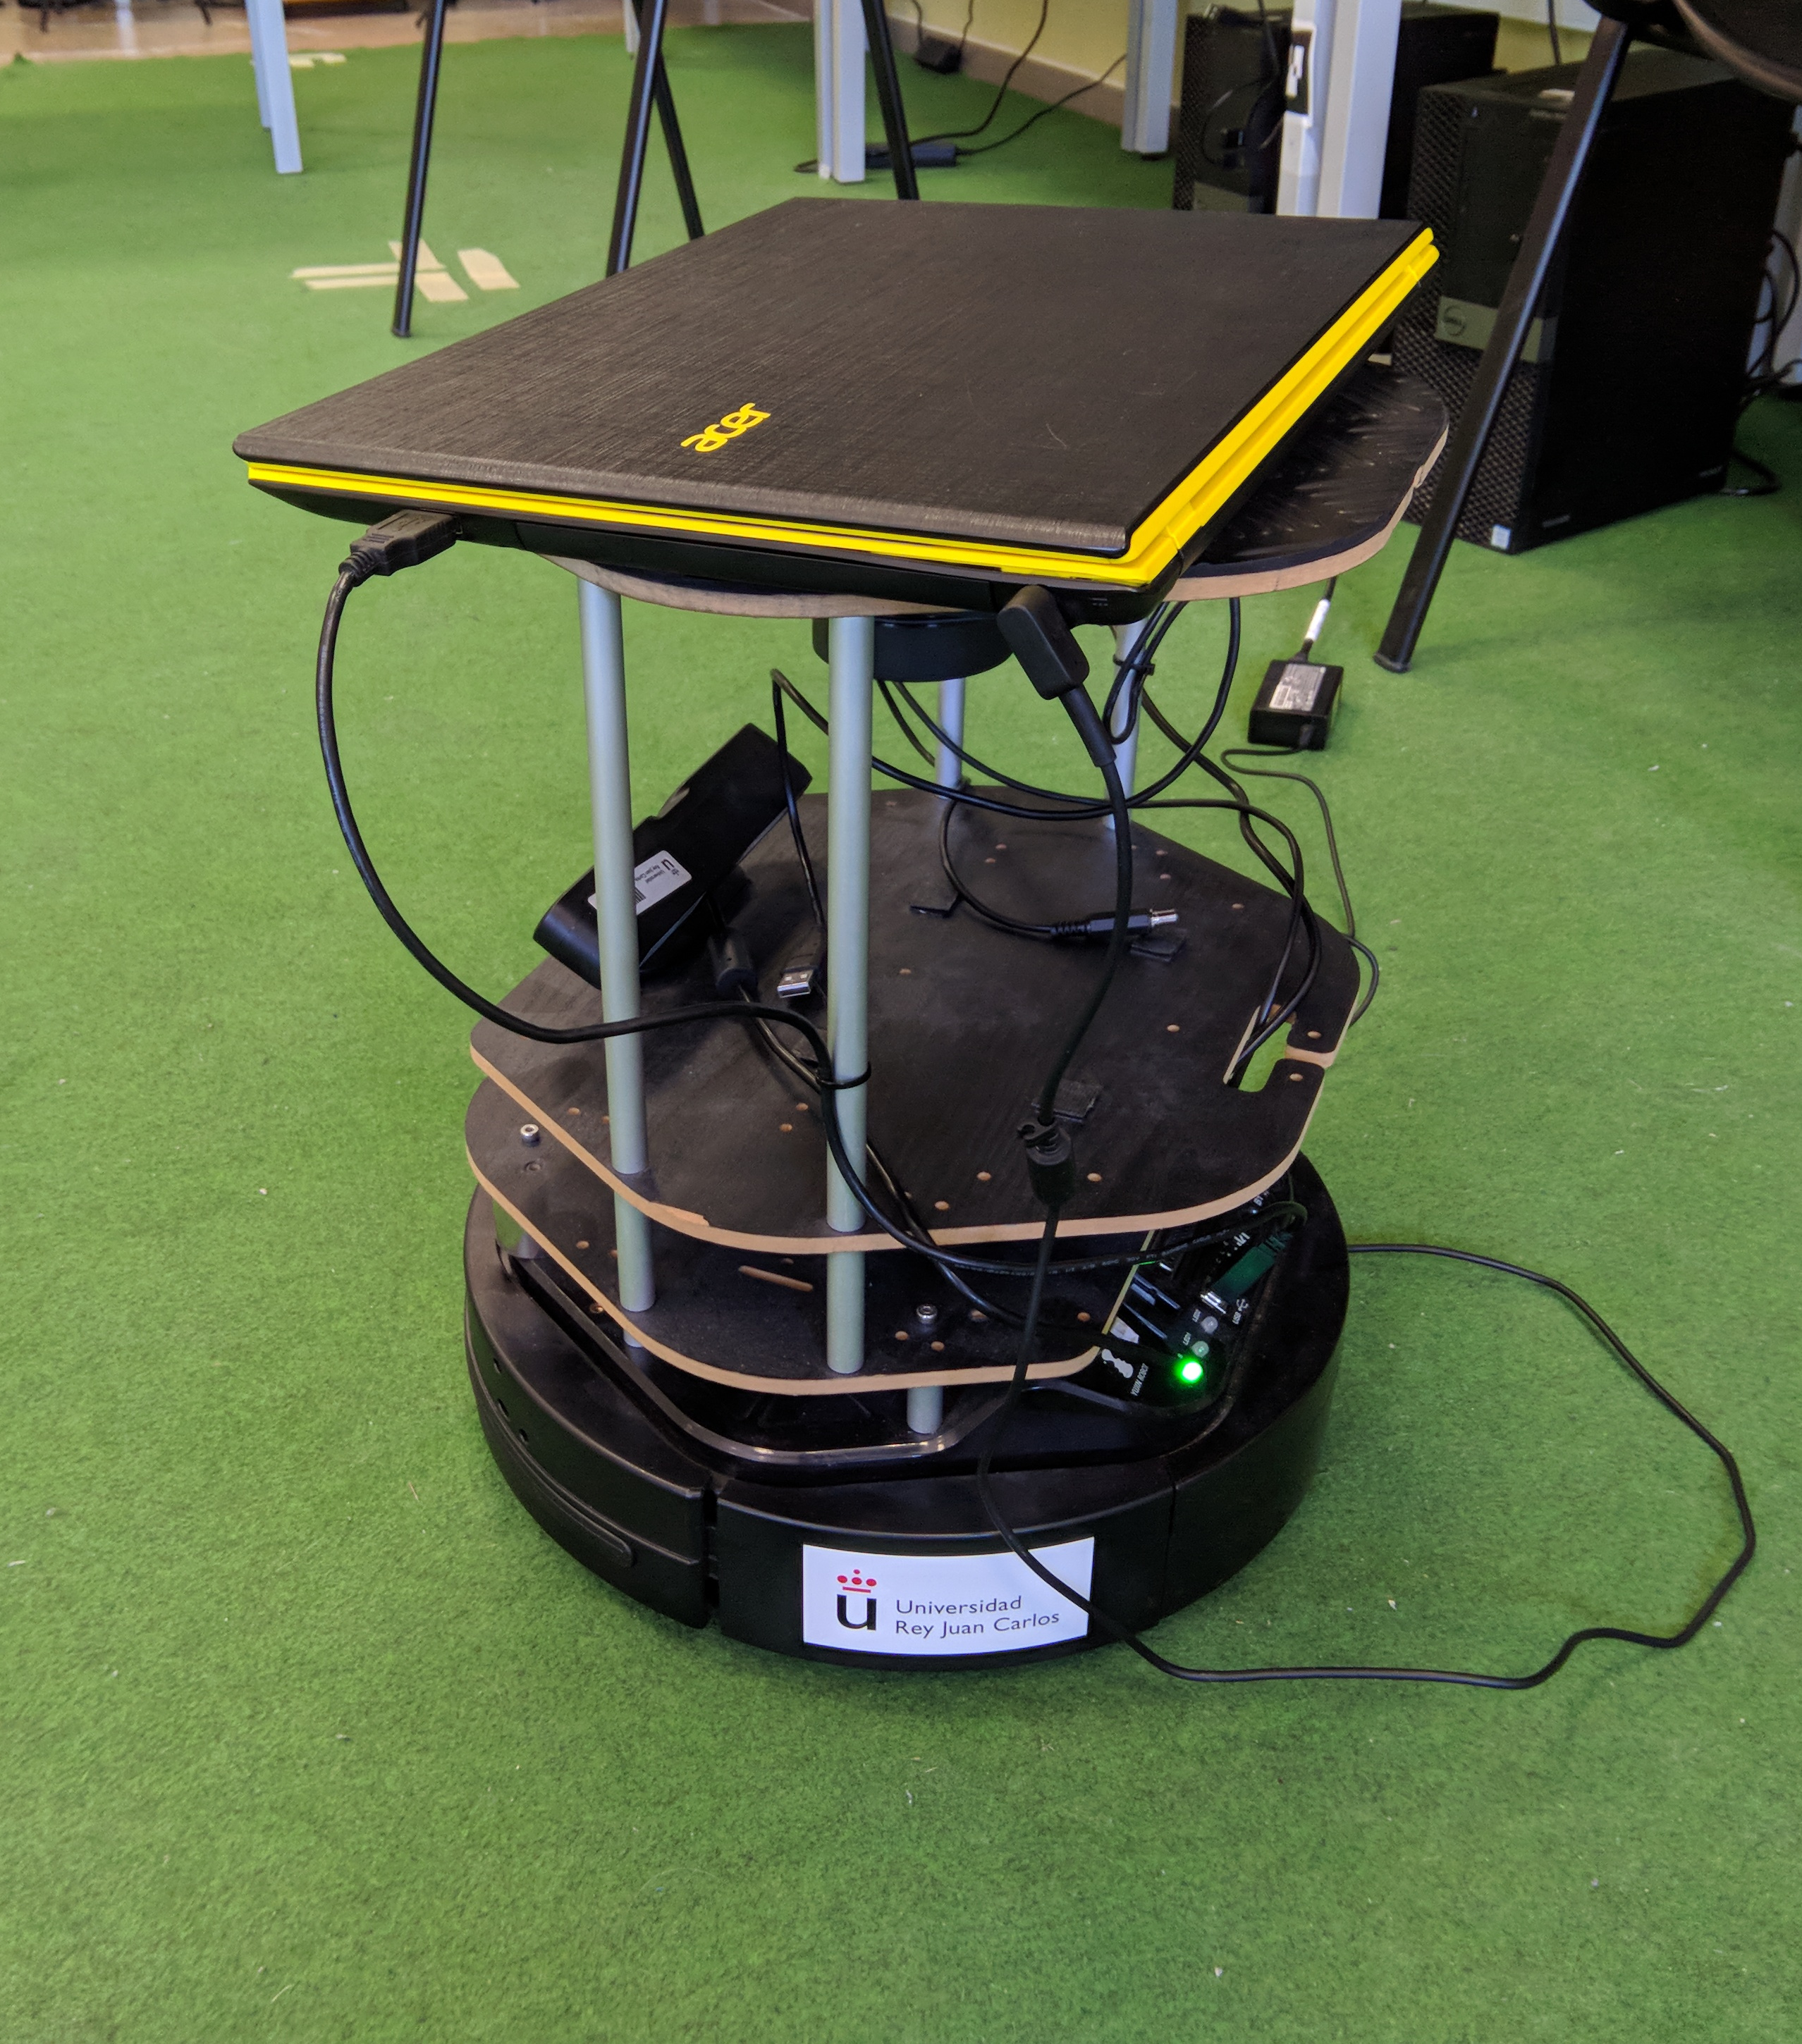
\includegraphics[width=2.2in]{tfg2}
		\caption{Side view.}
		\label{fig:2_turtlebot_side}
	\end{subfigure}
	\caption{Laptop+robot deployment on \cite{tfg}.}
	\label{fig:2_real_tfg}
\end{figure}

Nowadays, the mentioned increase in the interest into the real-time computer vision applications has fostered the development of specific low-power embedded devices to be integrated in mobile systems. The extending usage of devices such as Arduino or Raspberry Pi has led to embedded robotics systems, such as PiBot \cite{pibot} (\autoref{fig:2_pibot}). These robots are useful in the educational scope, as they are capable of running simple vision and navigation algorithms at a low cost.\\
\begin{figure}[h]
	\centering
	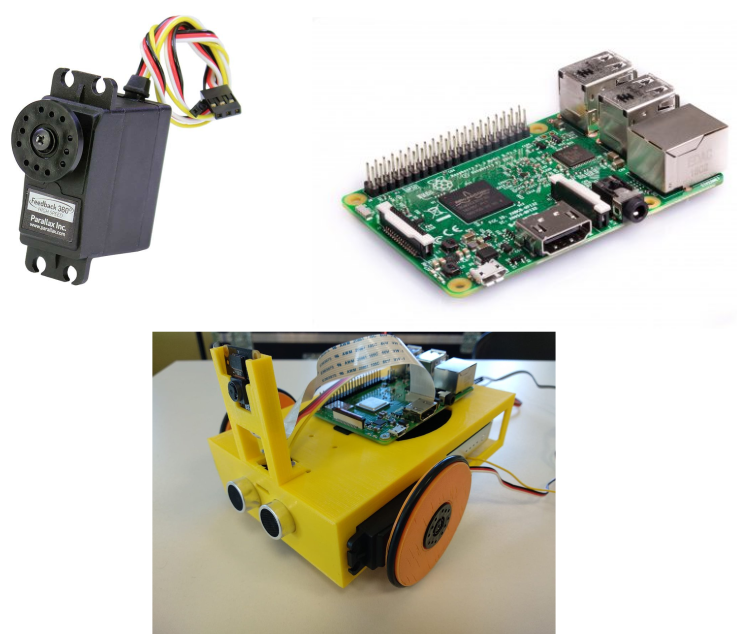
\includegraphics[width=0.5\linewidth]{pibot}
	\caption{PiBot, an open low-cost robotic platform for education (image from \cite{pibot}).}
	\label{fig:2_pibot}
\end{figure}
Unfortunately, the requirements for running more complex algorithms, such as neural networks, require of the next tier in power terms, keeping the portability nevertheless. The ideal device could be an ASIC (\textit{Application-Specific Integrated Circuit}), as the custom design would lead to a very tight optimization of the performance. However, the objective is to run the algorithms on existing software frameworks, requiring to use general purpose computers instead. The most remarkable advance in this scope are the Jetson devices manufactured by NVIDIA. These development boards are SoM computers running a tailored version of Linux. The fundamental feature of these systems is that they include a high-performance GPU featuring CUDA, a low-level parallel computation library, as well as several toolkits (such as TensorRT\footnote{\url{https://developer.nvidia.com/tensorrt}}) designed to optimize as much as possible the software implementations for the plethora of possibilities to be designed on this board. As it can be seen in \autoref{fig:2_tx2}, its size and power consumption make this system a good choice to be included in an autonomous robot. 
\begin{figure}[h!]
	\begin{subfigure}[h]{0.45\linewidth}
		\centering
		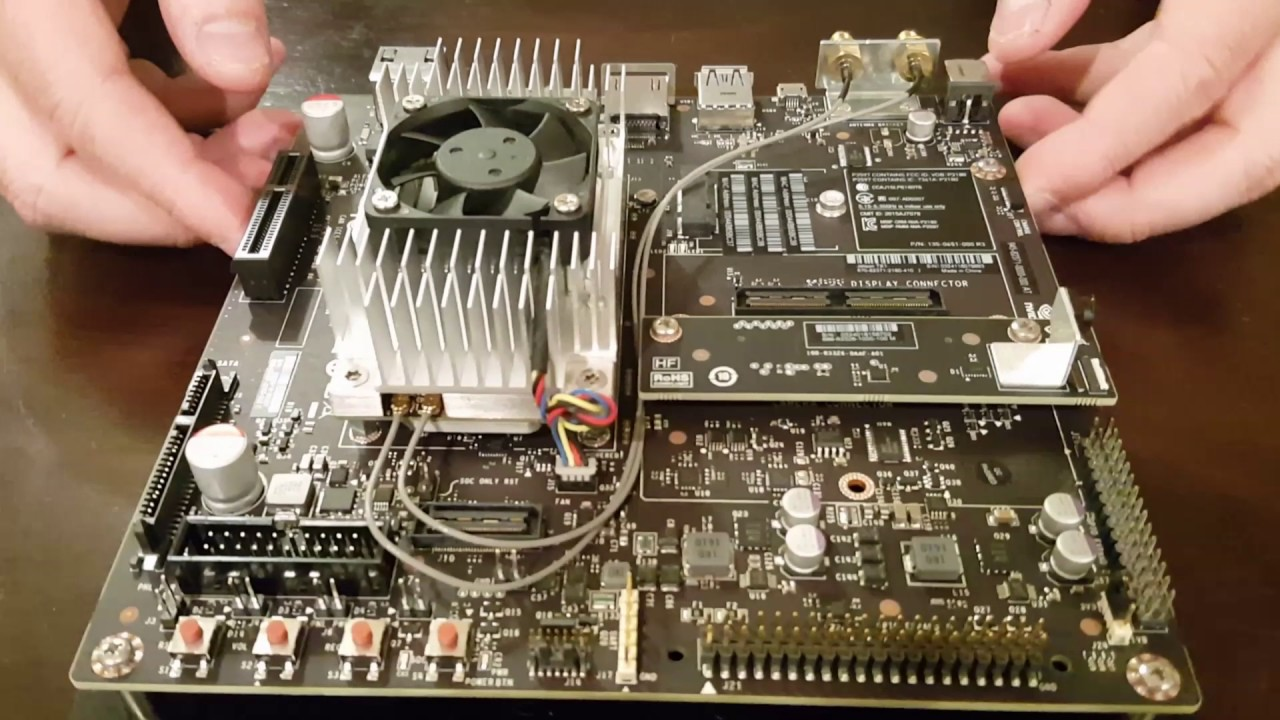
\includegraphics[width=\linewidth]{jetsontx2}

	\end{subfigure}
	\begin{subfigure}[h]{0.45\linewidth}
		\centering
		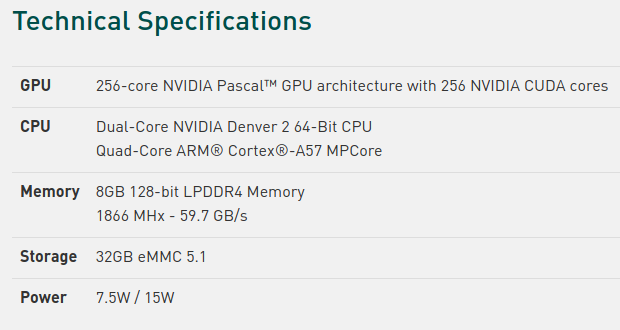
\includegraphics[width=\linewidth]{tx2_specs}
	\end{subfigure}
	\caption{NVIDIA Jetson TX2: an embedded high-performance device including a GPU.}
	\label{fig:2_tx2}
\end{figure}


\section{Person following}
\label{sec:2_following}
Several approaches have been developed pursuing this challenge of \textit{following a person}. Once the visual perception algorithms are established, the final output of the pipeline has to be a movement command for the robot to move towards the desired point. Mobile  robots can be classified according to their locomotion capabilities. A robot is \textit{holonomic} if the number of its controllable degrees of freedom is equal to its total degrees of freedom. If the controllable degrees of freedom are lower than the total degrees of freedom, the robot is \textit{non-holonomic}. This difference can be observed on \autoref{fig:2_holonomics}. In the case of a holonomic robot, the navigation process is simplified, as the robot can instantaneously move to a desired target. However, a non-holonomic robot needs to perform maneuvers in order to move towards a point.\\


\begin{figure}[h]
	\centering
	\begin{subfigure}[t]{0.45\linewidth}
		\centering
		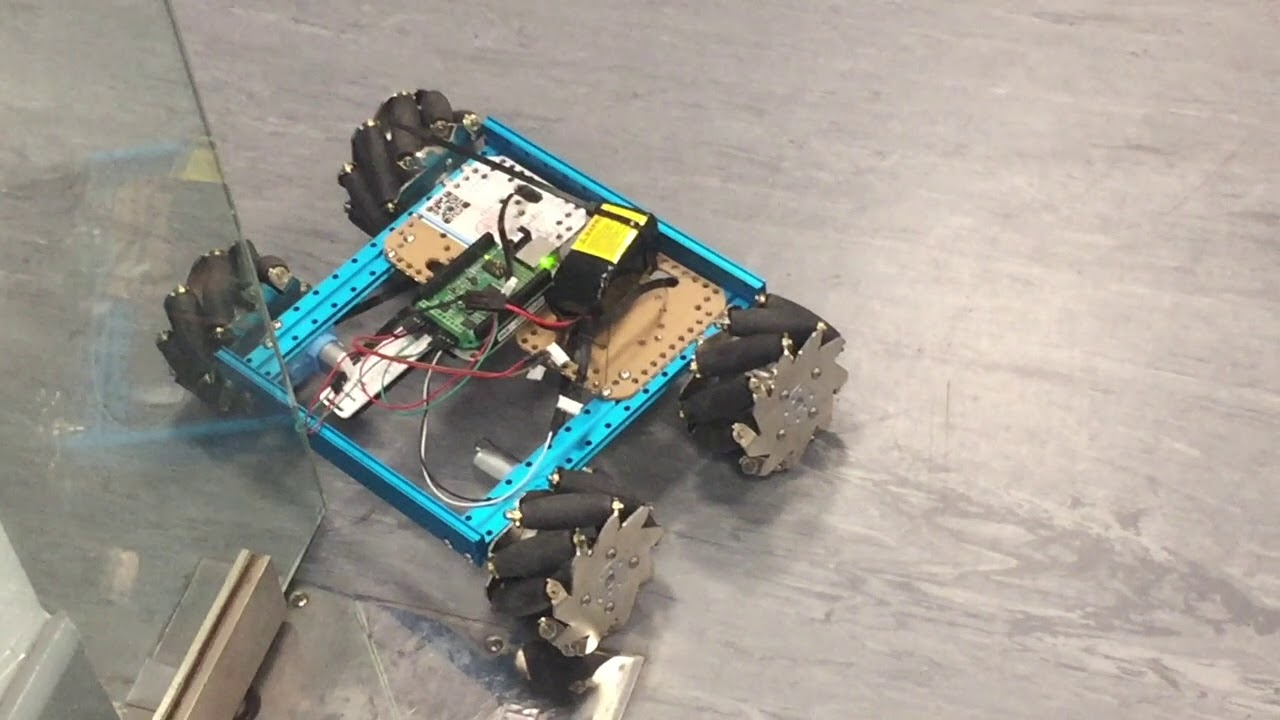
\includegraphics[width=\linewidth]{holonomic_robot}
		\caption{Holonomic robot.}
	\end{subfigure}
	\begin{subfigure}[t]{0.45\linewidth}
	\centering
	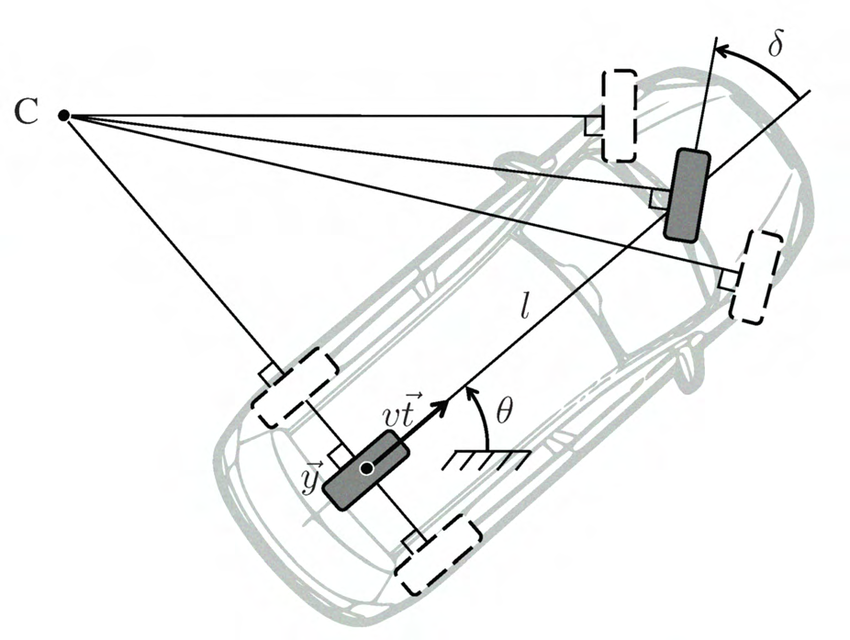
\includegraphics[width=\linewidth]{non_holonomic_robot}
	\caption{Schematic of the degrees of freedom of a non-holonomic vehicle (a standard car).}
	\end{subfigure}
	\caption{Comparison of a holonomic system with a non-holonomic one.}
	\label{fig:2_holonomics}
\end{figure}

The summary on \cite{personfollowing_summary} shows an interesting classification of some existing person following algorithms and their applications (\autoref{fig:2_personfollowing_summary}).


\begin{figure}[h]
	\centering
	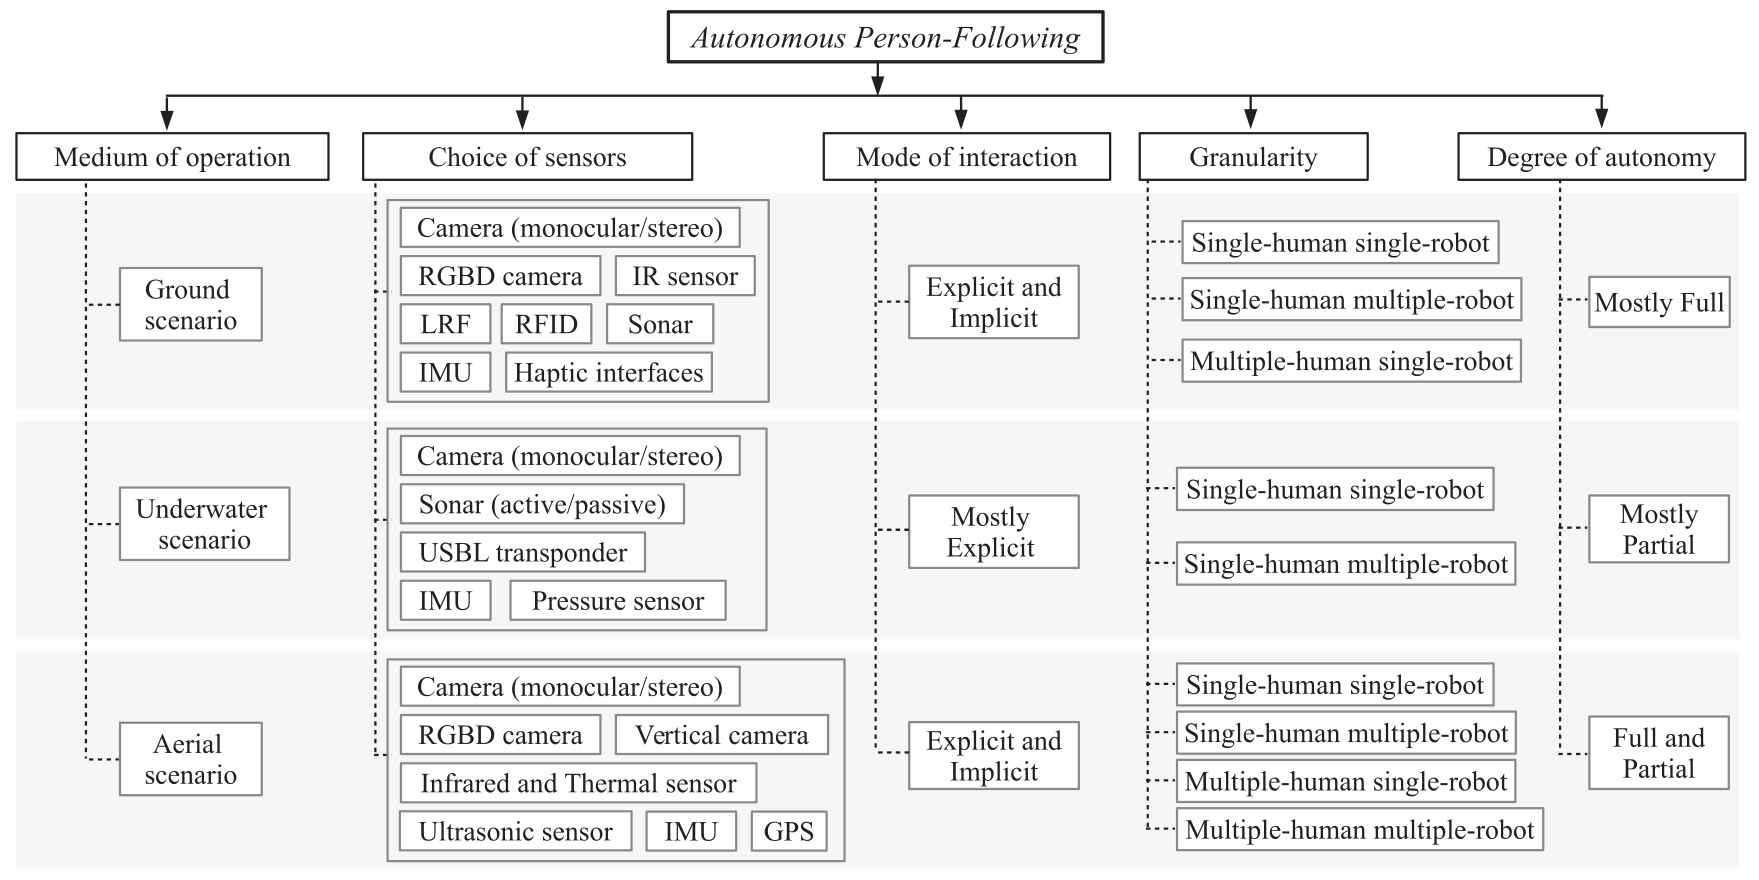
\includegraphics[width=\linewidth]{personfollowing_summary}
	\caption{In-depth classification of the existing person following algorithms (image from \cite{personfollowing_summary}).}
	\label{fig:2_personfollowing_summary}
\end{figure}

Some approaches leverage the detected objects in order to estimate the relative homography of the orthogonal planes, which allows to partially know the environment of the robot and trace a safe path towards the person, as it can be seen on \autoref{fig:2_personfollowing_homography}.

\begin{figure}
	\centering
	\begin{subfigure}[t]{0.45\linewidth}
		\centering
		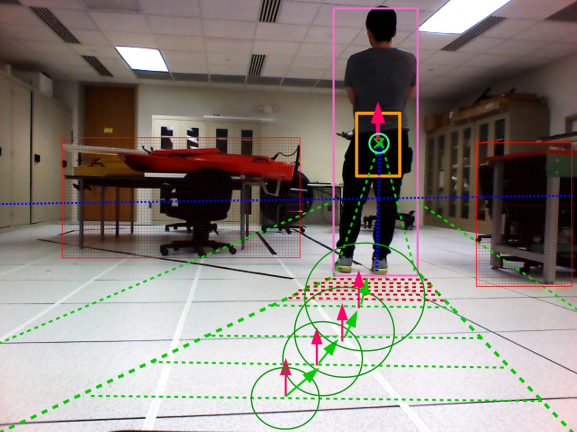
\includegraphics[width=0.95\linewidth]{personfollowing_homography}
		\caption{Following with path computation using homographies (image from \cite{personfollowing_summary}).}
		\label{fig:2_personfollowing_homography}
	\end{subfigure}
	\begin{subfigure}[t]{0.45\linewidth}
		\centering
		
		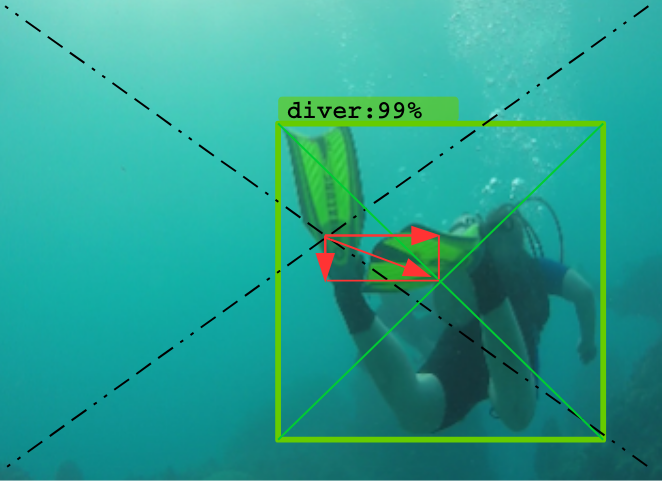
\includegraphics[width=0.95\linewidth]{personfollowing_reactive}
		\caption{Example of underwater reactive following (image from \cite{personfollowing_reactive}).}
		\label{fig:2_personfollowing_reactive}
	\end{subfigure}
	\caption{Examples of robotic following behavior.}
	\label{fig:2_personfollowing}
\end{figure}



Other approaches act without a path planning component, implementing what is called a \textit{reactive} behavior \cite{personfollowing_reactive}, similar to the proposed solution  on this work. On these approaches, the vector between the center of the image and the center of the person is used to command movements on the robot, as it can be seen on \autoref{fig:2_personfollowing_reactive}.
